\documentclass{article}
\usepackage{graphicx} % Required for inserting images
\usepackage{subcaption}
\usepackage{amsmath}
\usepackage{amssymb}
\usepackage{booktabs}

\title{SQUID \\
Advanced Physics Laboratory}
\author{Fynn Kanja 3780065 \\
Valentino D'Agosto 3763229 \\
Gruppe O43
}


\date{Experiment durchgeführt am: 12. Mai 2026}



\setlength{\parindent}{0pt}
\setlength{\parskip}{1em}
\usepackage[
    backend=biber,
    style=numeric,
  ]{biblatex}

\addbibresource{quellen.bib}



\begin{document}

\begin{figure}
    \centering
    
\includegraphics[width=0.75\linewidth]{uni_logo.png}
\end{figure}

\maketitle


\begin{abstract}

In diesem Experiment wird mit einem SQUID gearbeitet um kleinste Magnetfeldänderungen zu detektieren

\end{abstract}
\newpage
\begingroup
\tableofcontents
\endgroup
%\listoffigures
%\listoftables

\newpage

\section{Introduction}

\subsection{Aufgabestellung}
\begin{enumerate}
    \item Zusammen mit dem Betreuer führen Sie einen auf 77 K abgekühlten, massiven, schmelztexturierten Hochtemperatur-Supraleiter-Zylinder von oben in ein inhomogenes Magnetfeld aus 4 Permanentmagnetplatten ein. Beobachten Sie die Effekte bei der Erwärmung und erklären Sie diese anhand Ihrer Kenntnisse aus der Vorbereitung. Messen Sie den horizontalen und vertikalen Verlauf des Permanent-Magnetfeldes über den Platten mit einem Hallsensor.
    
    \item Spannungs-Strom-Messungen an einem DC-SQUID
    \begin{enumerate}
        \item Aufnehmen der V-I Kennlinie, Bestimmung des kritischen Stromes $2\times I_C$ des SQUID-Sensors, siehe Abb. V3 (Mr. SQUID guide S.10-13, Fig. 3-6)
        \item Bestimmung des Widerstandes im normalleitenden Zustand $R_N/2$ (normal state resistance), aus Steigung V-I, Abb. V4 (Mr. Squid guide S.13, Fig. 3-7) \cite{mr_squid}
        \item Bestimmung der charakteristischen Spannung als Produkt $I_C \times R_N \sim 100 - 200$ $\mu$V
    \end{enumerate}
    
    \item Shapiro-Stufen-Messung ($V$-$I$-Messung mit Mikrowellen-Einkopplung), Bestimmung von $e/h$ aus den Messungen (Mr. SQUID guide S. 72-77) \cite{mr_squid}
    
    \item $V$-$\phi$ Charakterisierung, Flux-locked-loop Messungen (FLL) (siehe auch Mr. SQUID guide S. 15 ff, und S. 27-28) \cite{mr_squid}
    \begin{enumerate}
        \item Bestimmung der maximalen Spannungsmodulation $\Delta V$ für ein Flussquant $\phi_0$, und der Induktivität $L$ des SQUID-Sensors, siehe unten S. 27 von Versuchsbeschreibung \cite{fprak_manual}
        \item Bestimmung des Modulationsparameters $\beta_L$ mit 2 verschiedenen Methoden, siehe S. 28 der Versuchsbeschreibung \cite{fprak_manual}
        \item Flussquantisierung in supraleitenden Ringen, Bestimmung des Zusammenhangs zwischen $V_{OUT}$ (SQUID) und dem vorhandenen magnetischen Fluss (siehe Advanced Experiments Section 7) \cite{mr_squid} 
    \end{enumerate}
    
    \item Bestimmen Sie die kritische Temperatur $T_c$ von $\text{YBa}_2\text{Cu}_3\text{O}_{7-\delta}$, dem Material des SQUID-Sensors näherungsweise, indem Sie die $I$-$V$-Kurve aus Aufgabe B) alle 1 K im Temperaturbereich von 77 K bis ca. 100 K aufnehmen. Die Temperatur wird mit einer Halbleiterdiode detektiert und ausgelesen. Die Variation der Temperatur erfolgt durch sehr langsames Herausziehen (und Fixieren) des SQUID-Stabes aus dem flüssigen Stickstoff. (Mr. SQUID guide S. 57-63 und S. 78-84) \cite{mr_squid}
\end{enumerate}







\subsection{Theoretische Grundlagen}

\subsubsection{Supraleitung}

Supraleitung ist ein makroskopisches Quantenphänomen, dass in Materialien auftritt, deren elektrischer Weiterstand bei einer bestimmten Sprungtemperatur $T_c$ praktisch null wird. Sie wurde von Heike Kamerlingh Onnes 1911 mittels einer stark gekühlten Quecksilber Probe ($T_C \gtrsim 0\mathrm{K}$) entdeckt. Wegen der Aufwendigkeit, die Probe so stark herunterzukühlen wurde erst ungefähr 20 Jahre später in 1933 der Meißner-Ochsenfeld-Effekt, von Walther Meißner und Robert Ochsenfeld, gezeigt. Nochmal 15 Jahre weiter, gab es eine theoretische Erklärung der Supraleitung mit der BCS-Theorie, welche 1957 von Bardeen, Cooper und Schrieffer aufgestellt wurde. Die Flussquantisierung in supraleitenden Ringen, welches, dass Hauptprinzip der SQUID Sensoren ist, nochmal gute 20 Jahre später theoretisch vorhergesagt und in 1961 experimentell bestätigt. \cite{mr_squid} \cite{fprak_manual}

Nach der Entdeckung von Hochtemperatur-Supraleiter, wurden Supraleiter viel alltagstauglicher für, dass handelsübliche Labor, da sie nicht mehr mit flüssigem Helium, sondern mit flüssigem Stockstoff heruntergekühlt werden welcher wesentlich günstiger ist \cite{liquid_he_na_prices}.

In der heutigen Zeit gibt es tausende von Materialien welche supraleitende Eigenschaften besitzen. Grob kann man diese in Supraleiter Typ I und Typ II aufteilen. (Mittels des Meißner Effekts)

\paragraph{Supraleiter Typ I}

Bei diesem Typen wird ein äußeres Magnetfeld vollständig aus dem Inneren des Supraleiters entfernt, bis auf deine dünne Oberflächenschicht, des Materials. Dort nimmt das Magnetfeld stark exponentiell ab, die dicke dieser Oberflächenschicht wird (Londonsche) Eindringtiefe genannt und befindet sich in einem ungefähren Bereich von ungefähr $100 \mathrm{nm}$. \cite{wiki-superconducter}. Dieser Zustand wird als Meißner Phase bezeichnet, die unterhalb der kritischen Temperatur auftritt $T<T_c$ wie in Abbildung \ref{fig:meißner_ochsnefeld_effekt} zu sehen ist.

\begin{figure}
    \centering
    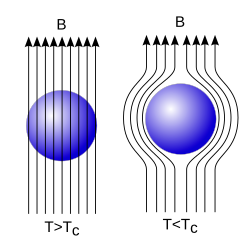
\includegraphics[width=0.5\linewidth]{figures/meißner_ochsenfeld_effekt.png}
    \caption{Der Meißner-Ochsenfeld-Effekt, als Eigenschaft von Supraleitern Typ. 1 in der Meißner Phase, ein von außen angelegtes magnetisches Feld vollständig aus dem Inneren zu verdrängen. Der Supraleiter ist somit nicht nur ein idealer Leiter ohne Widerstand, sondern auch ein idealer Diamagnet. \cite{wiki-meissner-ochsenfeld}}
    \label{fig:meißner_ochsnefeld_effekt}
\end{figure}

Wichtig zu erwähne ist, dass der Supraleitende Zustand nicht allein von der Temperatur abhängig ist. Auch unterhalb der kritischen Temperatur $T < T_c$ kann ein Supraleiter 1. Art normal leitend werden und so einen nicht vernachlässigbar kleinen Widerstand besitzen. Dazu kommt es, wenn entweder dass äußere Magnetfeld einen kritischen Wert $B_c$ oder die Stromdichte durch den Supraleiter einen kritischen Wert $J_c$ überschreitet. \cite{wiki-superconducter}

\paragraph{Cooper-Paare}
Die Supraleitung von Typ-I-Supraleitern wird durch die Bildung sogenannter Cooper-Paare erklärt. In einem gewöhnlichen elektrischen Leiter bewegen sich Elektronen durch das Kristallgitter des Materials. Dabei werden sie an Gitterfehlern und an thermischen Gitterschwingungen, den sogenannten Phononen, gestreut. Diese Streuprozesse verursachen den elektrischen Widerstand.

Unterhalb der kritischen Temperatur verändert sich dieses Verhalten grundlegend. Ein Elektron, das sich durch das Kristallgitter bewegt, zieht aufgrund seiner negativen Ladung die positiv geladenen Atomrümpfe geringfügig an. Dadurch entsteht lokal für kurze Zeit eine erhöhte positive Ladungsdichte. Da die Atomrümpfe deutlich schwerer und somit träger sind als die Elektronen, folgt ihre Bewegung verzögert und diese Gitterverzerrung bleibt für einen kurzen Moment bestehen. Ein zweites Elektron kann von dieser positiven Ladungsdichte angezogen werden, da sich die Atomrümpfe noch in Richtung der ursprünglichen Position des ersten Elektrons verschoben haben. In diesem Bereich ist die Dichte der positiv geladenen Atomrümpfe daher kurzzeitig erhöht, wodurch für das zweite Elektron eine anziehende Wirkung entsteht. Auf diese Weise entsteht eine indirekte, durch Phononen vermittelte Anziehung zwischen zwei Elektronen.

Ist diese Anziehung stärker als die elektrische Coulomb-Abstoßung, bilden die beiden Elektronen ein gebundenes Paar, das als Cooper-Paar bezeichnet wird. Die Elektronen eines Cooper-Paares besitzen entgegengesetzte Impulse und entgegengesetzten Spin. Dadurch beträgt der Gesamtimpuls und der Gesamtspin des Paares jeweils null.

Mikroskopisch erstreckt sich ein Cooper-Paar nicht nur über wenige Atomabstände, sondern über viele tausend Gitterabstände. Die beiden Elektronen sind daher nicht als eng gebundenes Teilchenpaar zu verstehen, sondern als ein gemeinsamer quantenmechanischer Zustand, bei dem die Aufenthaltswahrscheinlichkeiten der Elektronen über einen großen Bereich des Kristallgitters verteilt sind. Obwohl die Elektronen räumlich weit voneinander entfernt sein können, bleiben sie durch die phonenvermittelte Wechselwirkung miteinander gekoppelt und verhalten sich wie eine Einheit.

Da sich die Wellenfunktionen vieler Cooper-Paare stark überlappen, können sie nicht mehr als voneinander unabhängige Paare betrachtet werden. Stattdessen befinden sich sehr viele Cooper-Paare gleichzeitig im selben makroskopischen Quantenzustand und bilden ein gemeinsames Kondensat. Dieses Kondensat wird durch eine einzige kohärente Wellenfunktion beschrieben, sodass sich alle Cooper-Paare gemeinsam und geordnet durch das Kristallgitter bewegen. Gerade diese kollektive Bewegung ist eine wesentliche Voraussetzung für das widerstandsfreie Fließen des elektrischen Stroms.
 \cite{demtroder_3} \cite{fprak_manual} \cite{wiki-superconducter} \cite{wiki-cooper}

\paragraph{Supraleiter Typ II}

Supraleiter des Typs II verhalten sich bis zu einem \textit{unteren kritischen Magnetfeld} $B_{c1}$ in der Meißner Phase und verhalten sich somit analog zu Supraleiter des Typs I. Ist, dass äußere Magnetfeld aber höher als $B_{c1}$, so können die magnetischen Feldlinien in der Form von Flussschläuchen in, dass Material eindringen. Dabei kann der magnetischer Fluss $\Phi$, in solch einem Schlauch, immer nur gleich dem magnetischen Flussquants sein. \cite{fprak_manual} \cite{wiki-superconducter}
Da durch den gesamten Supraleiter nur eine ganzzahlige Anzahl, solche Flussschläuche durchlaufen, ist der gesamte magnetische Fluss ein ganzzahliges Vielfaches des magnetischen Flussquants.

\begin{equation}
    \Phi_0 = \frac{h}{2e} \approx 2.07 \times 10^{-15} \mathrm{Vs}
\end{equation}

Ist das äußere Magnetfeld noch stärker und oberhalb des \textit{oberen kritischen Magnetfeldes} $B_{c2}$ ist der supraleitende Zustand nicht mehr vorhanden.

Theoretisch sind Supraleiter zweiter Art nicht so gut verstanden wie die, der erster Art. Es wird angenommen, dass auch bei diesen Supraleitern es zur Bildung von Cooper Paaren kommt. Jedoch konnte noch kein allgemein akzeptiertes Modell gefunden werden, dass diese Supraleiter vollständig beschreiben kann. Die Entdeckung eines solchen Modells wäre sehr interessant, da alle Hochtemperatur-Supraleiter, die meisten supraleitenden Legierungen und Eisen-Pniktide Supraleiter der zweiten Art sind.

\subsubsection{Supraleitende Ringe}
Die Basis eines Squid Sensores ist ein Supraleitender Ring

\subsubsection{Josephson-Effekt}

\subsubsection{SQUID Sensor}

\subsection{Experimenteller Aufbau}

Für den ersten Teil des Experimentes, wurde ein auf 77 K abgekühlten, massiven, schmelztexturierten Hochtemperatur-Supraleiter-Zylinder in ein, aus einer Fläche von 4 Paramagneten erzeugtes, inhomogenes Magnetfeld eingebracht. Für den zweiten Teil wurde ein mit flüssigem Stickstoff gefülltes Kryostat benutzt in dem der SQUID Sensor drin war.

\begin{figure}
    \centering
    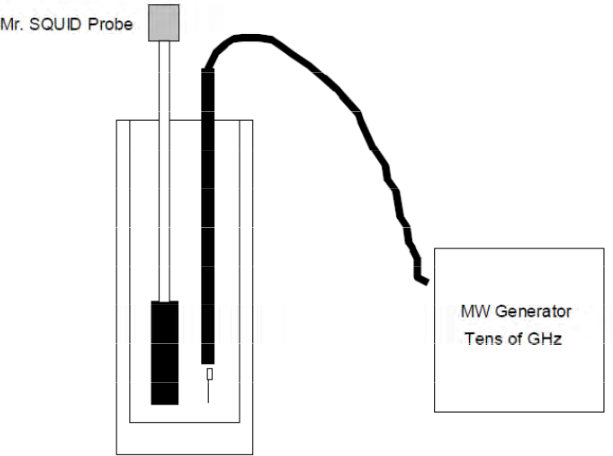
\includegraphics[width=0.5\linewidth]{figures/schematischer_versuchsaufbau.png}
    \caption{Schematischer Versuchsaufbau, der Aufgabe 3 zur Bestimmung der Shapiro-Stufen. Mit der Mr. Squid Probe und der verbundenen $\lambda/4$ Antenne im Kryostaten, der mit flüssigen Stickstoff gefüllt ist. Versuchsaubau für Aufgabe 2, 4 und 5 sehr analog, nur ohne die $\lambda/4$ Antenne.}
    \label{fig:versuchsaubau}
\end{figure}

\section{Ergebnisse und Diskussion}

\subsection{Hochtemperatur-Supraleiter im inhomogenen Magnetfeld}

\subsubsection{Ermittlung des horizontalen und vertikalen Verlauf des Permanent-Magnetfeldes}

Zu Beginn wurde das Magnetfeld der vier Permanentmagnetplatten mithilfe eines Hallsensors untersucht. Dazu wurde die magnetische Flussdichte einmal horizontal über die Magnetanordnung und einmal vertikal in Abhängigkeit vom Abstand zur Oberfläche aufgenommen. Das Magnetfeld ist, wie der horizontale Verlauf verdeutlicht, inhomogen und weist Bereiche mit unterschiedlicher Feldstärke und wechselnder Polarität auf. Der vertikale Verlauf zeigt erwartungsgemäß, dass die magnetische Flussdichte abnimmt, je weiter man sich von den Magnetplatten entfernt.

\begin{figure}
    \centering
    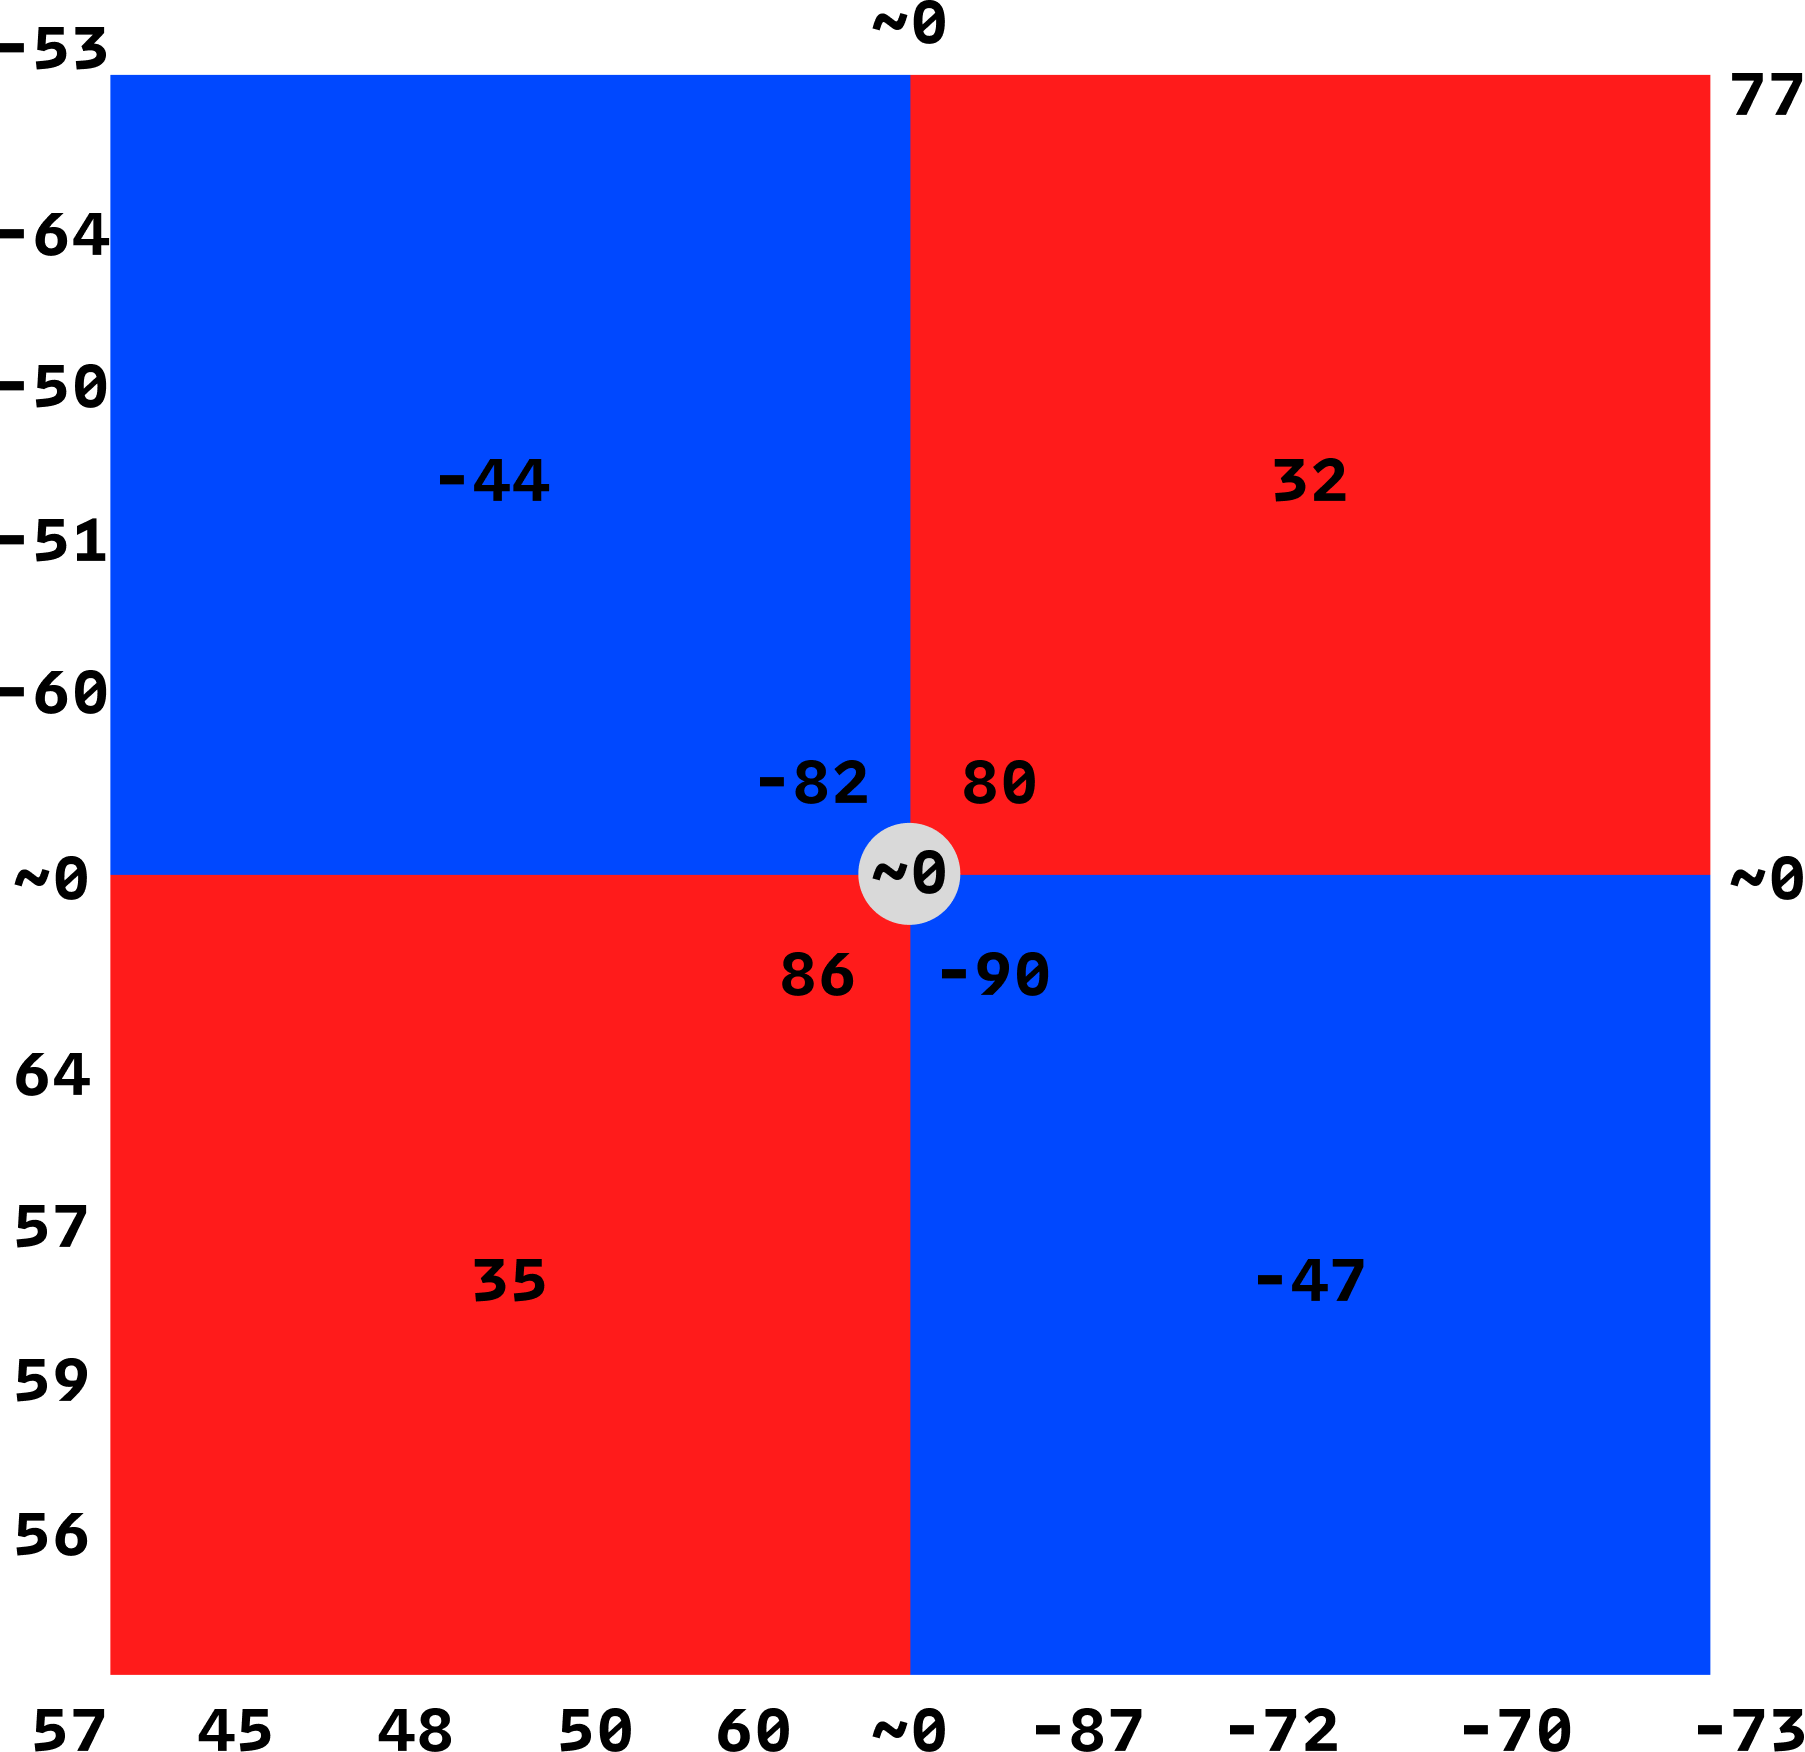
\includegraphics[width=0.75\linewidth]{figures/magnetische_ausrichtugn_4magnete.png}
    \caption{Alle Zahlen, sind in den EInheiten mT gemessen wurden}
    \label{fig:mag_ausr_4mag}
\end{figure}

\subsubsection{Hochtemperatur-Supraleiter-Zylinder im inhomogneen Magnetfeld}

Anschließend wurde ein auf 77 K gekühlter Hochtemperatur-Supraleiter-Zylinder von oben in das Magnetfeld eingebracht. Dabei konnte ein Schwebezustand beobachtet werden. Dieser lässt sich durch den Meißner-Ochsenfeld-Effekt erklären: Im supraleitenden Zustand werden Magnetfeldlinien aus dem Inneren des Supraleiters verdrängt, wodurch im inhomogenen Magnetfeld eine abstoßende bzw. stabilisierende Kraft entsteht. Da es sich um einen Typ-II-Supraleiter handelt, können zusätzlich Flussschläuche und Pinning-Effekte zur Stabilisierung beitragen. Beim Erwärmen überschreitet der Körper nach einiger Zeit die kritische Temperatur, sodass der supraleitende Zustand verloren geht und der Schwebezustand endet.

\begin{figure}
    \centering
    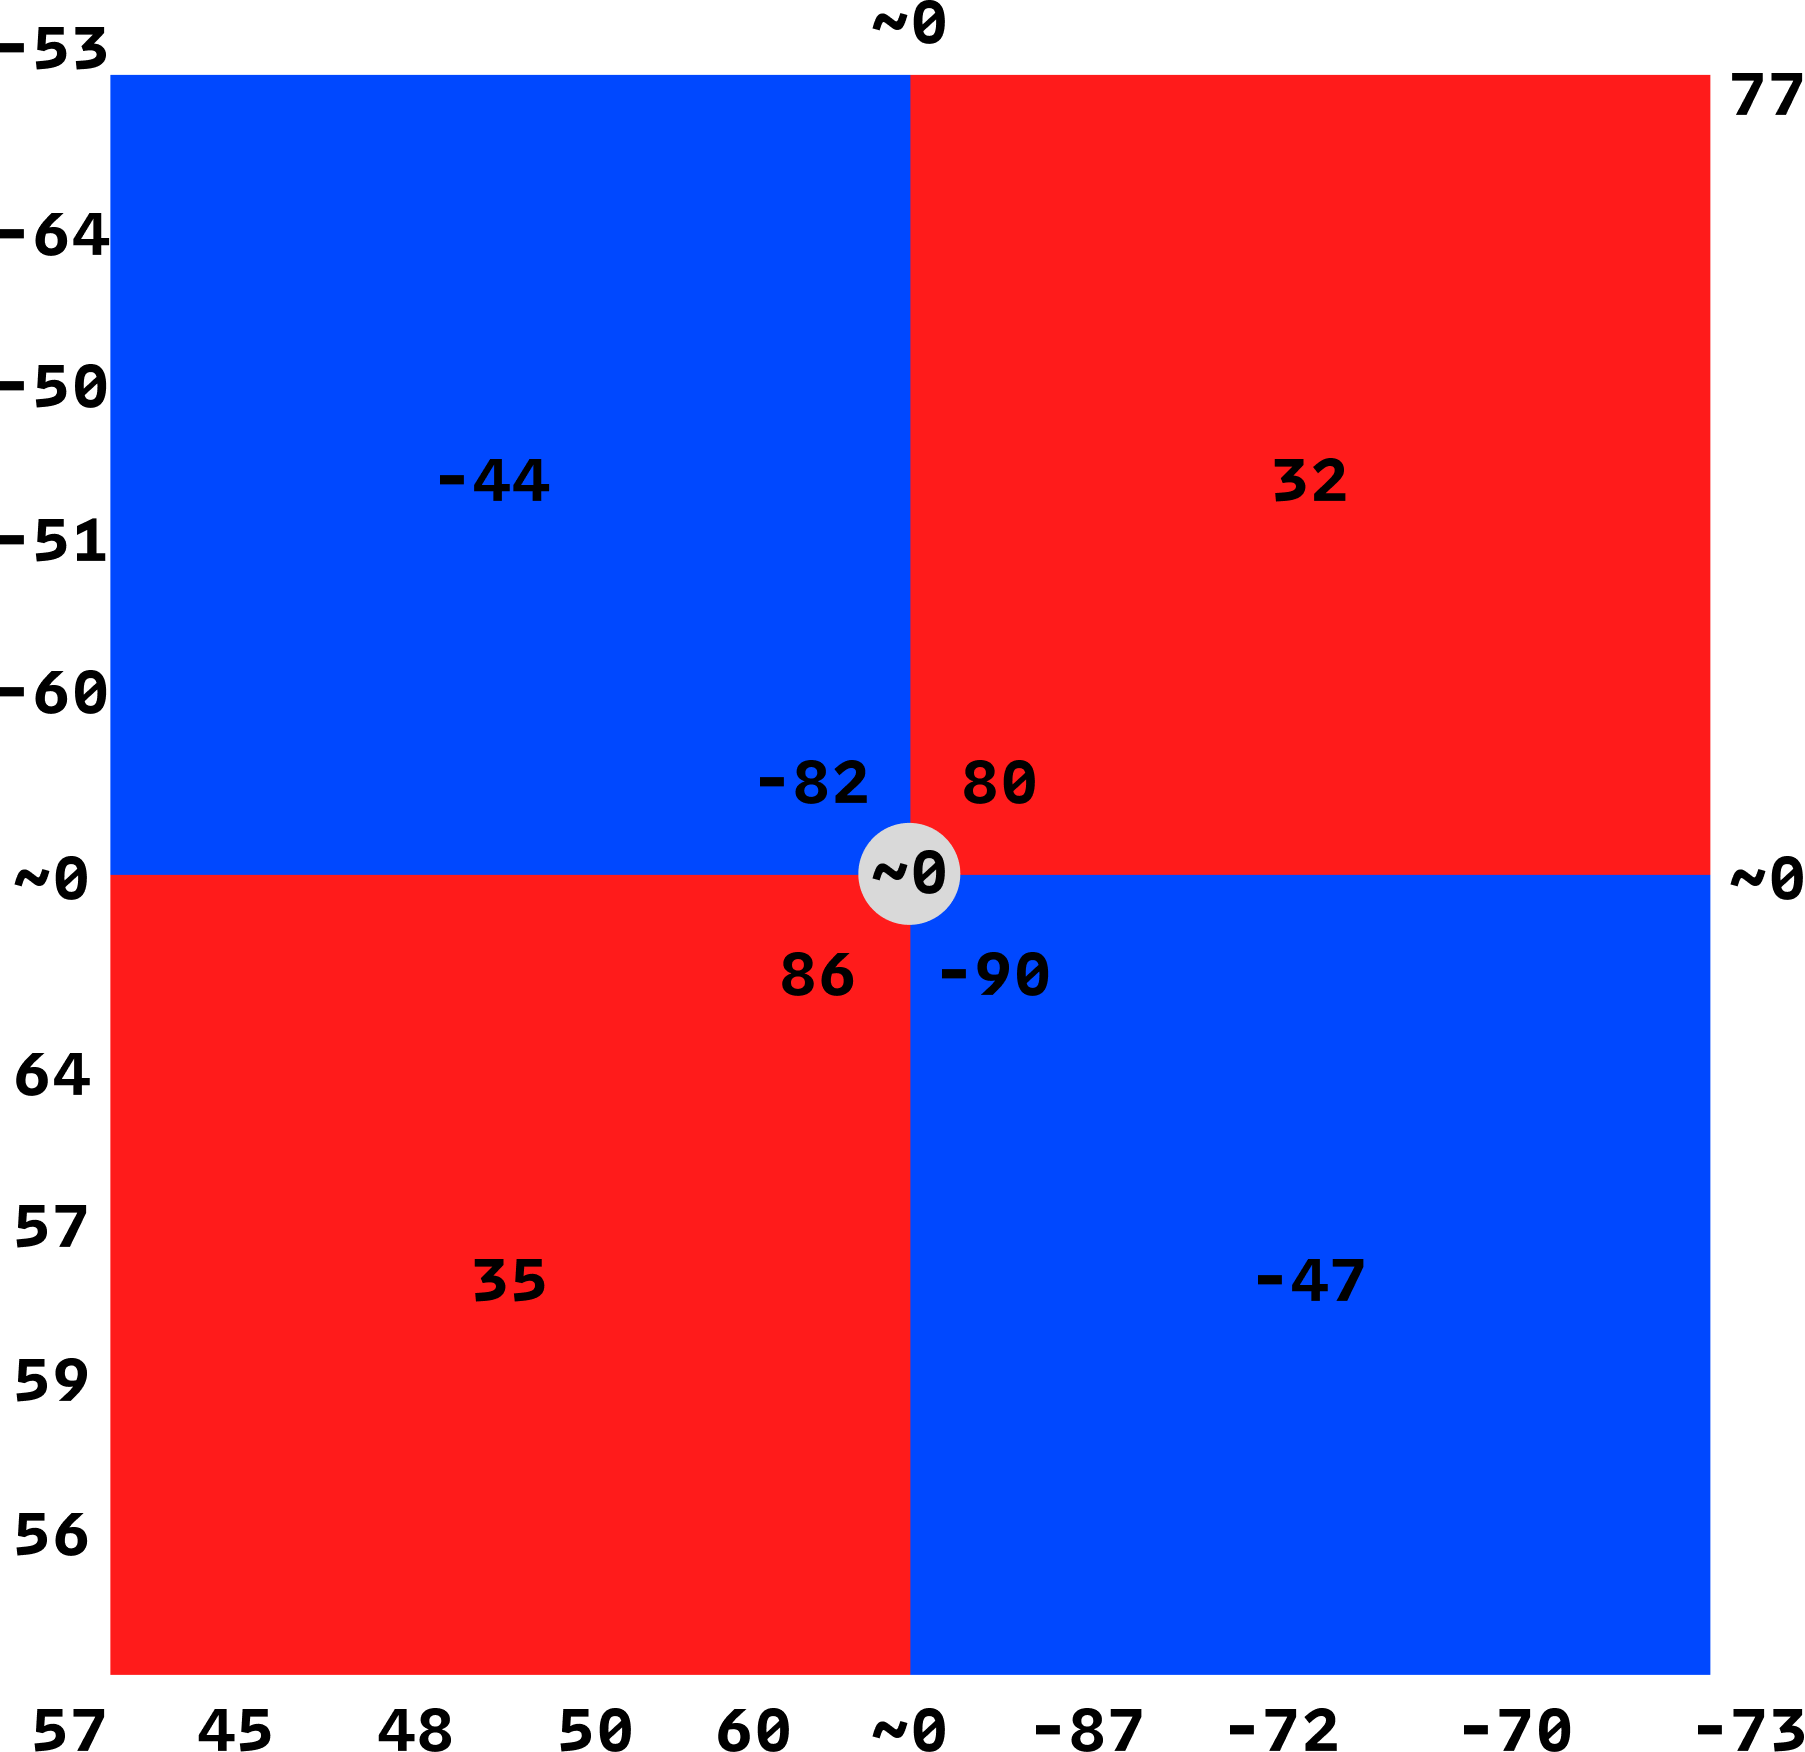
\includegraphics[width=0.75\linewidth]{figures/magnetische_ausrichtugn_4magnete.png}
    \caption{Supraleiter im inhomogenen Magnetfeld}
    \label{fig:supraleiter_auf_inhom_magnetfeld}
\end{figure}

Auffällig war, dass der supraleitende Zylinder nicht an jeder Position über der Magnetanordnung stabil schwebte, sondern vor allem im zentralen Bereich des inhomogenen Magnetfeldes. Dies lässt sich durch die Symmetrie der vier Permanentmagnetplatten erklären. In der Mitte kompensieren sich die horizontalen Kraftkomponenten weitgehend, während die vertikale magnetische Kraft den Zylinder gegen die Gewichtskraft stabilisieren kann. An den Übergängen zwischen Bereichen positiver und negativer Feldrichtung ist das Magnetfeld dagegen stark inhomogen. Da verschiedene Bereiche des Supraleiters dort unterschiedlich gerichtete Magnetfeldkomponenten erfahren, entstehen neben der vertikalen Kraft auch Drehmomente. Diese führen dazu, dass der Zylinder eine schräge Gleichgewichtslage einnimmt. Die beobachtete Schrägstellung ist somit eine Folge der starken Feldgradienten und der unsymmetrischen Kraftverteilung an den Magnetübergängen. Der stabile Schwebezustand in der Mitte wird zusätzlich durch Flusspin­ning im Typ-II-Hochtemperatur-Supraleiter begünstigt.

\subsection{Spannungs-Strom-Messungen an einem DC-SQUID}

In dieser Aufgabe wurde die Spannungs-Strom-Kennlinie des DC-SQUIDs aufgenommen. Die Kennlinie zeigt im Bereich um $I=0$ einen nahezu spannungsfreien Zustand. Dies entspricht dem DC-Josephson-Effekt, bei dem ein Suprastrom ohne messbare Spannung durch die Josephson-Kontakte fließt. Erst bei Überschreiten des kritischen Stroms geht der SQUID in einen spannungsbehafteten, näherungsweise ohmschen Zustand über.

Zur Bestimmung des kritischen Stroms wurden die linearen Bereiche der positiven $I_{0+}$ und negativen Flanke $I_{0-}$ separat gefittet. Aus den Schnittpunkten der Fitgeraden mit der Stromachse ergaben sich

\begin{equation}
    I_{0+} = 51.0 \mathrm{µA} \qquad \text{und} \qquad I_{0-} = -48.8 \mathrm{µA}
\end{equation}

Da der SQUID aus zwei parallelen Josephson-Kontakten besteht, entspricht der kritische Strom des gesamten SQUIDs dem Wert $2I_c$. Aus dem Mittelwert der Beträge folgt

\begin{equation}
    2I_C = \frac{|I_{0+} - I_{0-}|}{2} = \frac{|51.0 - (-48.8)|}{2} \mathrm{µA} = 49.9 \mathrm{µA}
\end{equation}

und so der finale Wert für $I_C = 24.95 \mathrm{µA}$.
Aus der Steigung der linearen Kennlinienbereiche wurde der Widerstand im normalleitenden Zustand $R_N/2 = 2.29 \Omega$ bestimmt. Daraus ergibt sich für den normalleitenden Widerstand eines einzelnen Josephson-Kontaktes $R_N = 4.58 \Omega$. Die charakteristische Spannung des SQUIDs, beträgt somit

\begin{equation}
    I_C \cdot R_N = 24.95 \mathrm{µA} \cdot 4.58 \Omega = 114.4 \mathrm{µV}
\end{equation}

Der erhaltene Wert liegt im erwarteten Bereich von etwa $100 - 200 \mathrm{µV}$. Die Messung ist damit gut mit der erwarteten Größenordnung für den verwendeten SQUID-Sensor verträglich.


\begin{figure}[h]
    \centering
    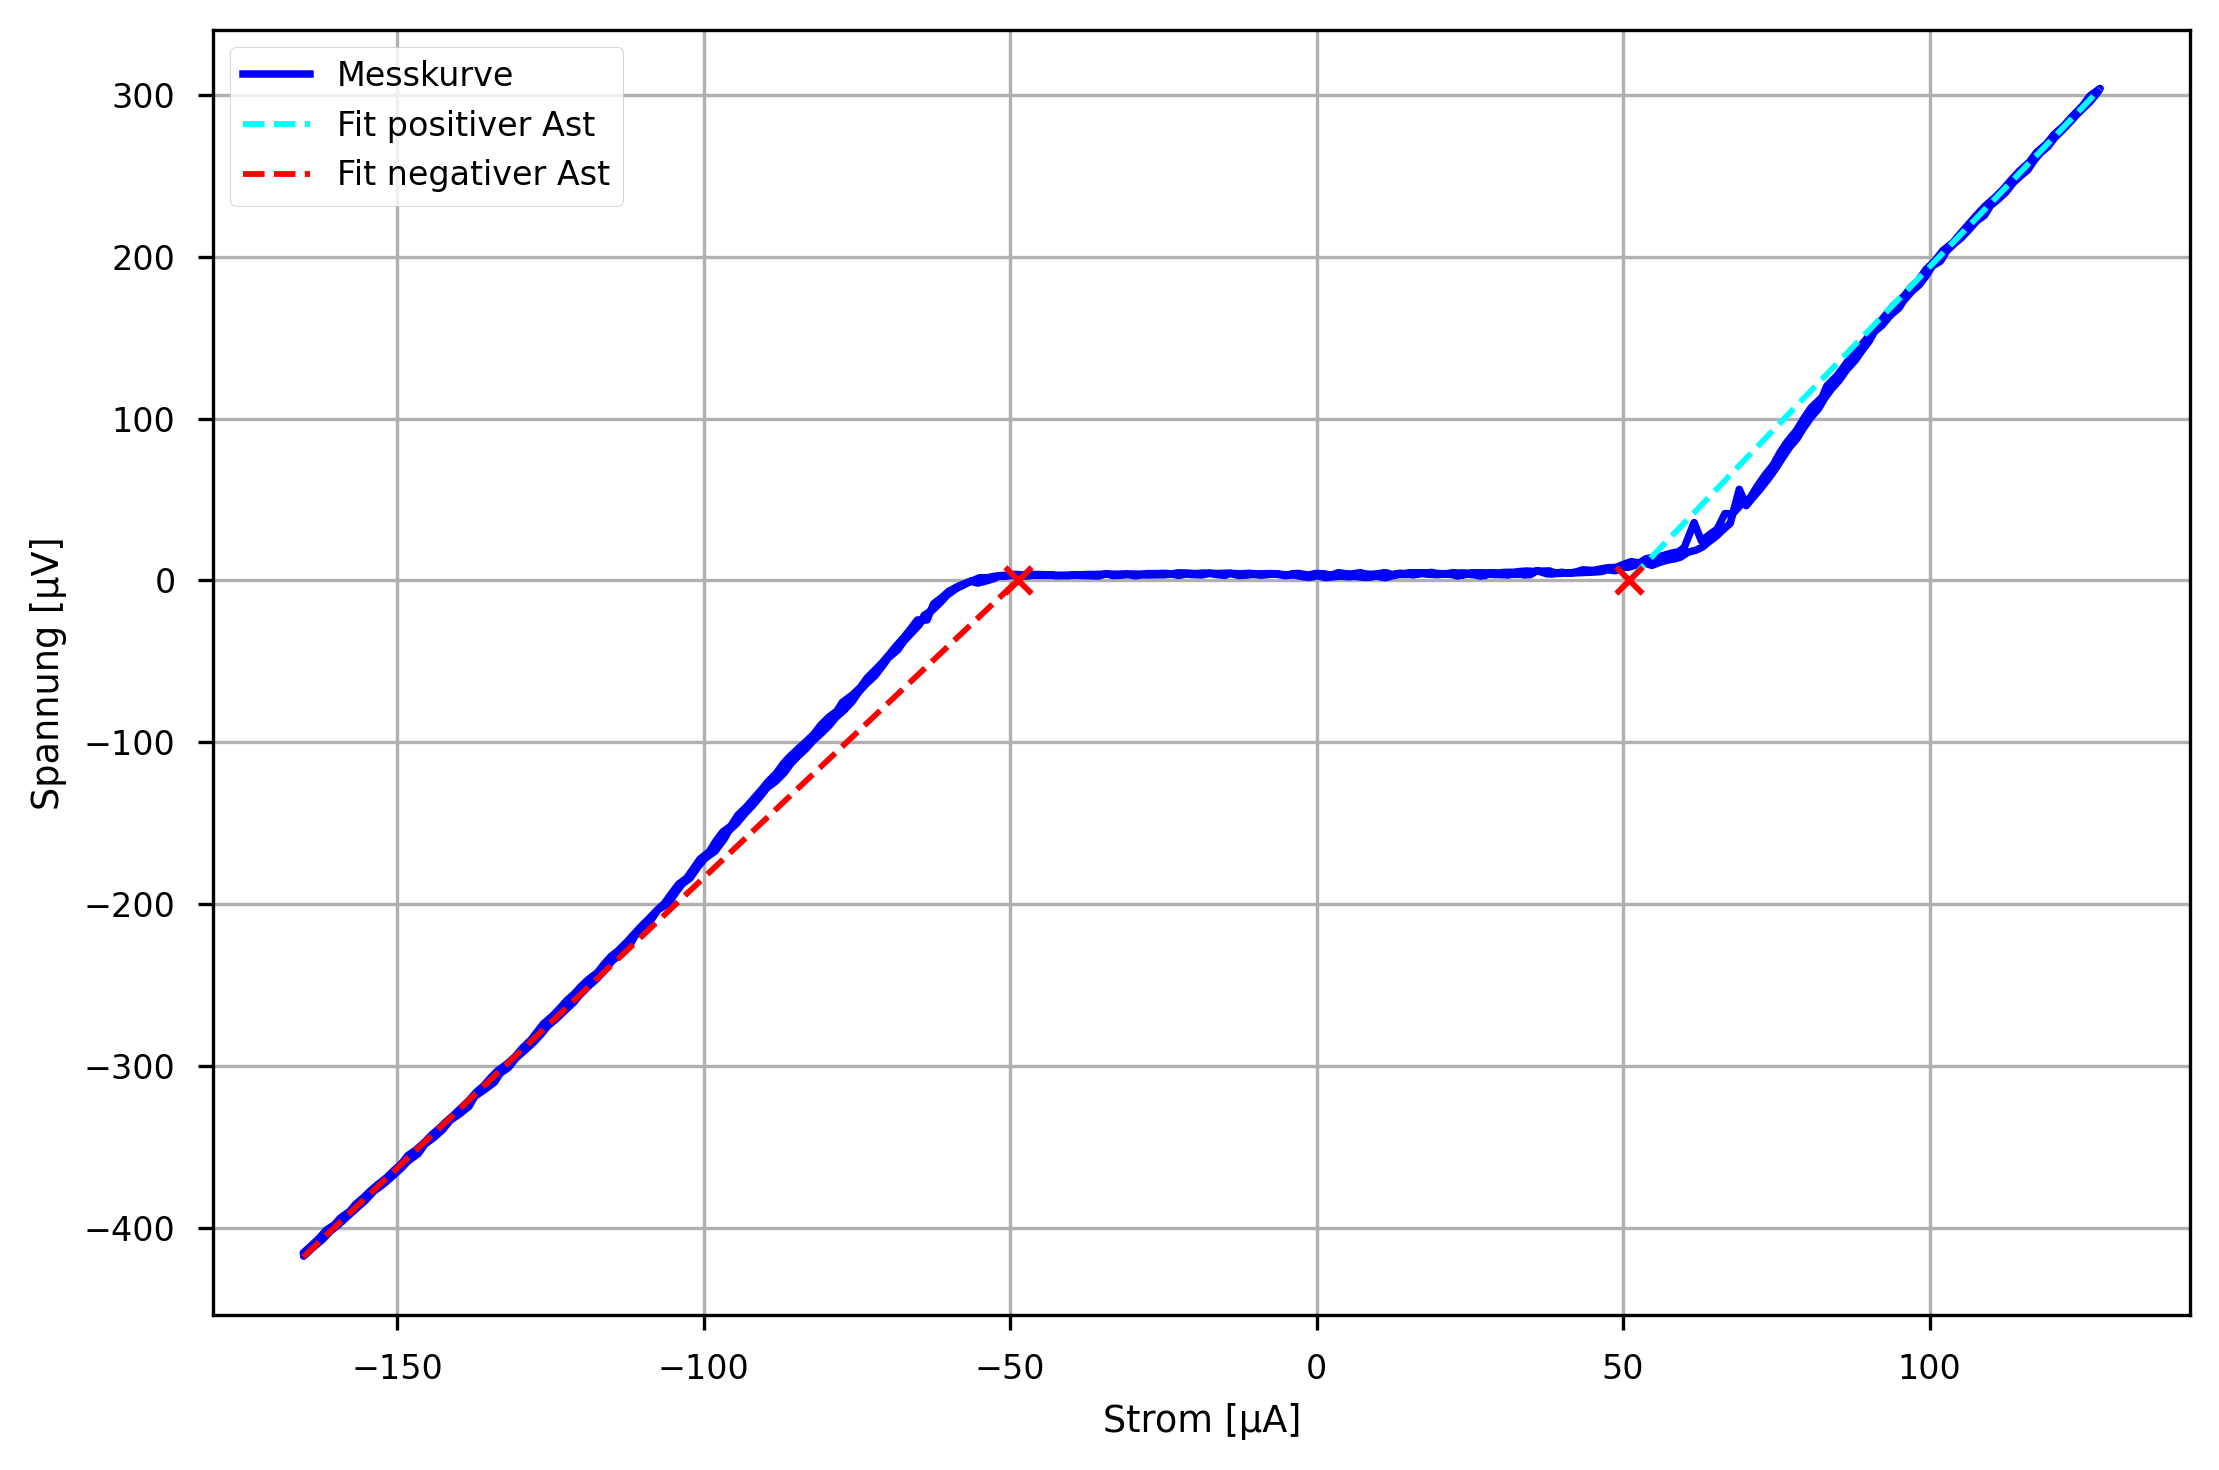
\includegraphics[width=0.75\linewidth]{figures/Aufgabe_B_Fit.png}
    \caption{Spannungs-Strom-Kennlinie des DC-SQUIDs mit linearer Extrapolation der positiven und negativen Kennlinienäste zur Bestimmung des kritischen Stroms $2I_C$. Die roten Punkte markieren die Schnittpunkte der Fitgeraden mit der Stromachse.}
    \label{fig:aufgabe_b_fit}
\end{figure}

\subsection{Shapiro-Stufen-Messung}

In Aufgabe C wurde die U-I-Kennlinie des DC-SQUIDs unter Einkopplung einer Mikrowelle mit der Frequenz $f = 44 \mathrm{GHz}$ aufgenommen. Durch die Wechselwirkung der externen Mikrowellenfrequenz mit der Josephson-Oszillation der Weak Links entstehen diskrete Spannungsplateaus, die sogenannten Shapiro-Stufen. Diese treten auf, wenn die Josephson-Frequenz mit der eingestrahlten Mikrowellenfrequenz synchronisiert wird.

\begin{figure}[h]
    \centering
    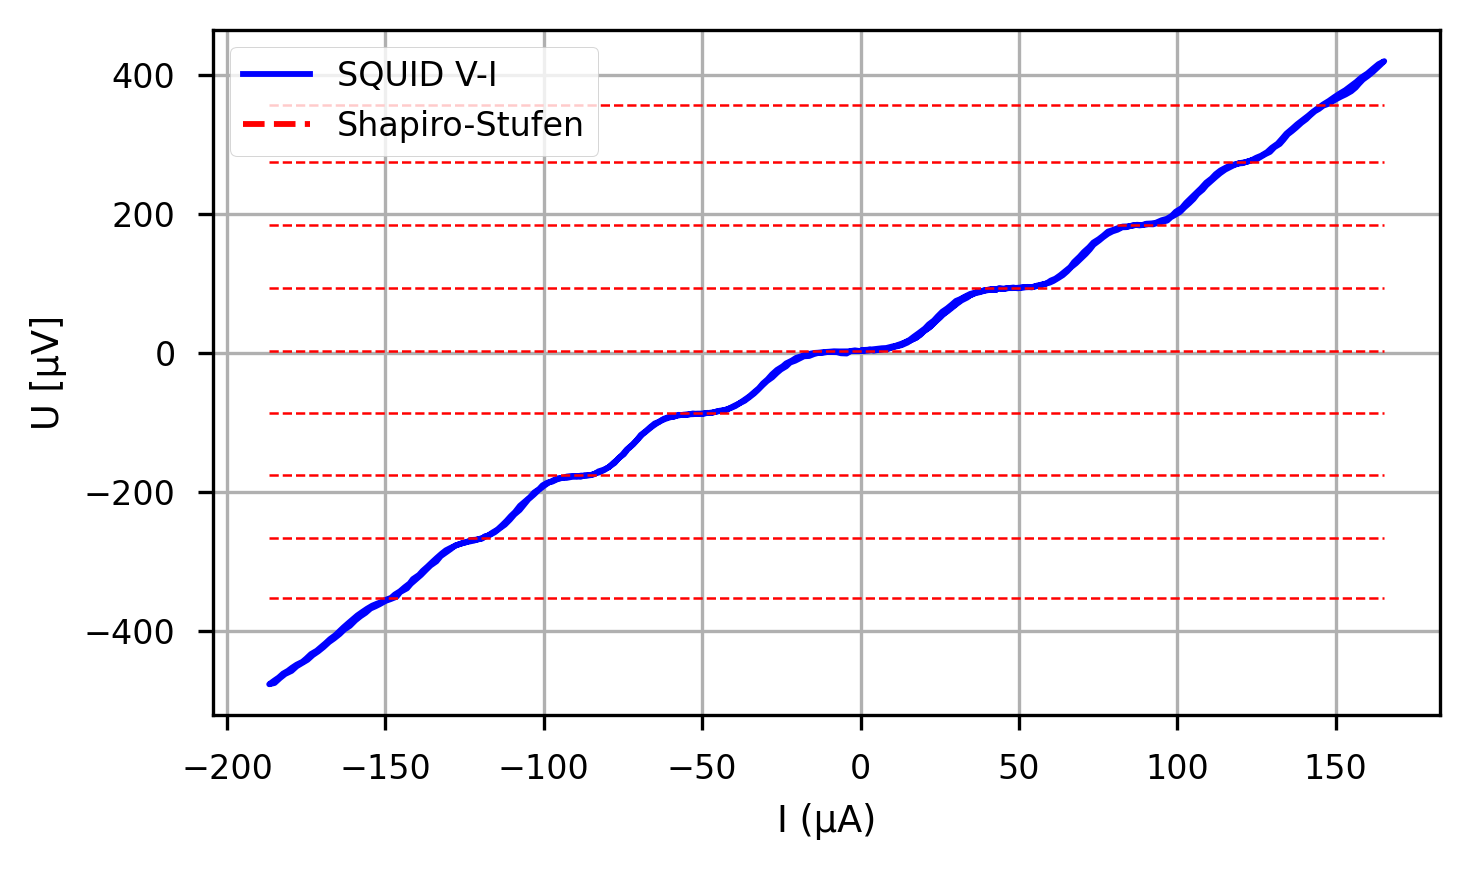
\includegraphics[width=0.75\linewidth]{figures/saphiero_stufen.png}
    \caption{U-I-Kennlinie des DC-SQUIDs bei Einkopplung einer Mikrowelle mit der Frequenz $f = 44 \mathrm{GHz}$. Die gestrichelten Linien markieren die bestimmten Shapiro-Stufen.}
    \label{fig:shapiro_stufen}
\end{figure}

Aus der U-I-Kennlinie \ref{fig:shapiro_stufen} wurden die Spannungspositionen der einzelnen Shapiro-Stufen bestimmt. Der mittlere Abstand benachbarter Stufen beträgt dabei $\Delta U = 88.625  \pm  1.10 \mathrm{µV}$. 

Aus der gemessenen mittleren Stufenspannung und der bekannten Frequenz der eingestrahlten Mikrowelle lässt sich die fundamentale Konstante $e/h$ bestimmen mit der für die Shapiro-Stufen geltende der Zusammenhang

\begin{equation}
    \Delta U = \frac{hf}{2e} \qquad \Leftrightarrow \qquad \frac{e}{h} = \frac{f}{2\Delta U}
\end{equation}

Unter Berücksichtigung der Unsicherheit des mittleren Stufenabstands und mit $f = 44 \mathrm{GHz}$ ergibt sich

\begin{equation}
    \frac{e}{h} = \frac{44 \cdot 10^9 \mathrm{Hz}}{2 \cdot 88.625 \cdot 10^{-6} \mathrm{V}} = 2.48 \pm 0.03 \mathrm{Hz/mV}
\end{equation}

Damit weicht der experimentell bestimmte Wert um etwa 2.7\% vom Literaturwert ab. Die Abweichung ist plausibel und kann durch die endliche Breite der Shapiro-Stufen, Rauschen der Messkurve, Unsicherheiten bei der Bestimmung der Stufenpositionen sowie eine nicht ideale Mikrowellenkopplung erklärt werden.

\subsection{$V$-$\Phi$ Charakterisierung}

In Aufgabe D wurde die $U_{OUT}$-$I$-Kennlinie des DC-SQUIDs aufgenommen. Dabei wurde die Ausgangsspannung $U_{OUT}$ in Abhängigkeit vom Spulenstrom I gemessen. Da der Spulenstrom proportional zum magnetischen Fluss durch den SQUID-Ring ist, entspricht die periodische Modulation der Ausgangsspannung der $V$-$\Phi$-Charakteristik des SQUIDs. Eine vollständige Periode der Kurve entspricht dabei einer Änderung des magnetischen Flusses um ein Flussquant \Phi_0$.

Die Messdaten \ref{fig:aufgabe_d} zeigen eine deutlich periodische Modulation der Ausgangsspannung. Aufgrund des sichtbaren Rauschens und eines leichten linearen Drifts wurde die Kennlinie nicht mit einer einfachen Sinusfunktion, sondern mit einer Sinusfunktion mit zusätzlichem linearen Driftterm gefittet wie in  \ref{fig:aufgabe_d} zu sehen ist.

\begin{figure}[h]
    \centering
    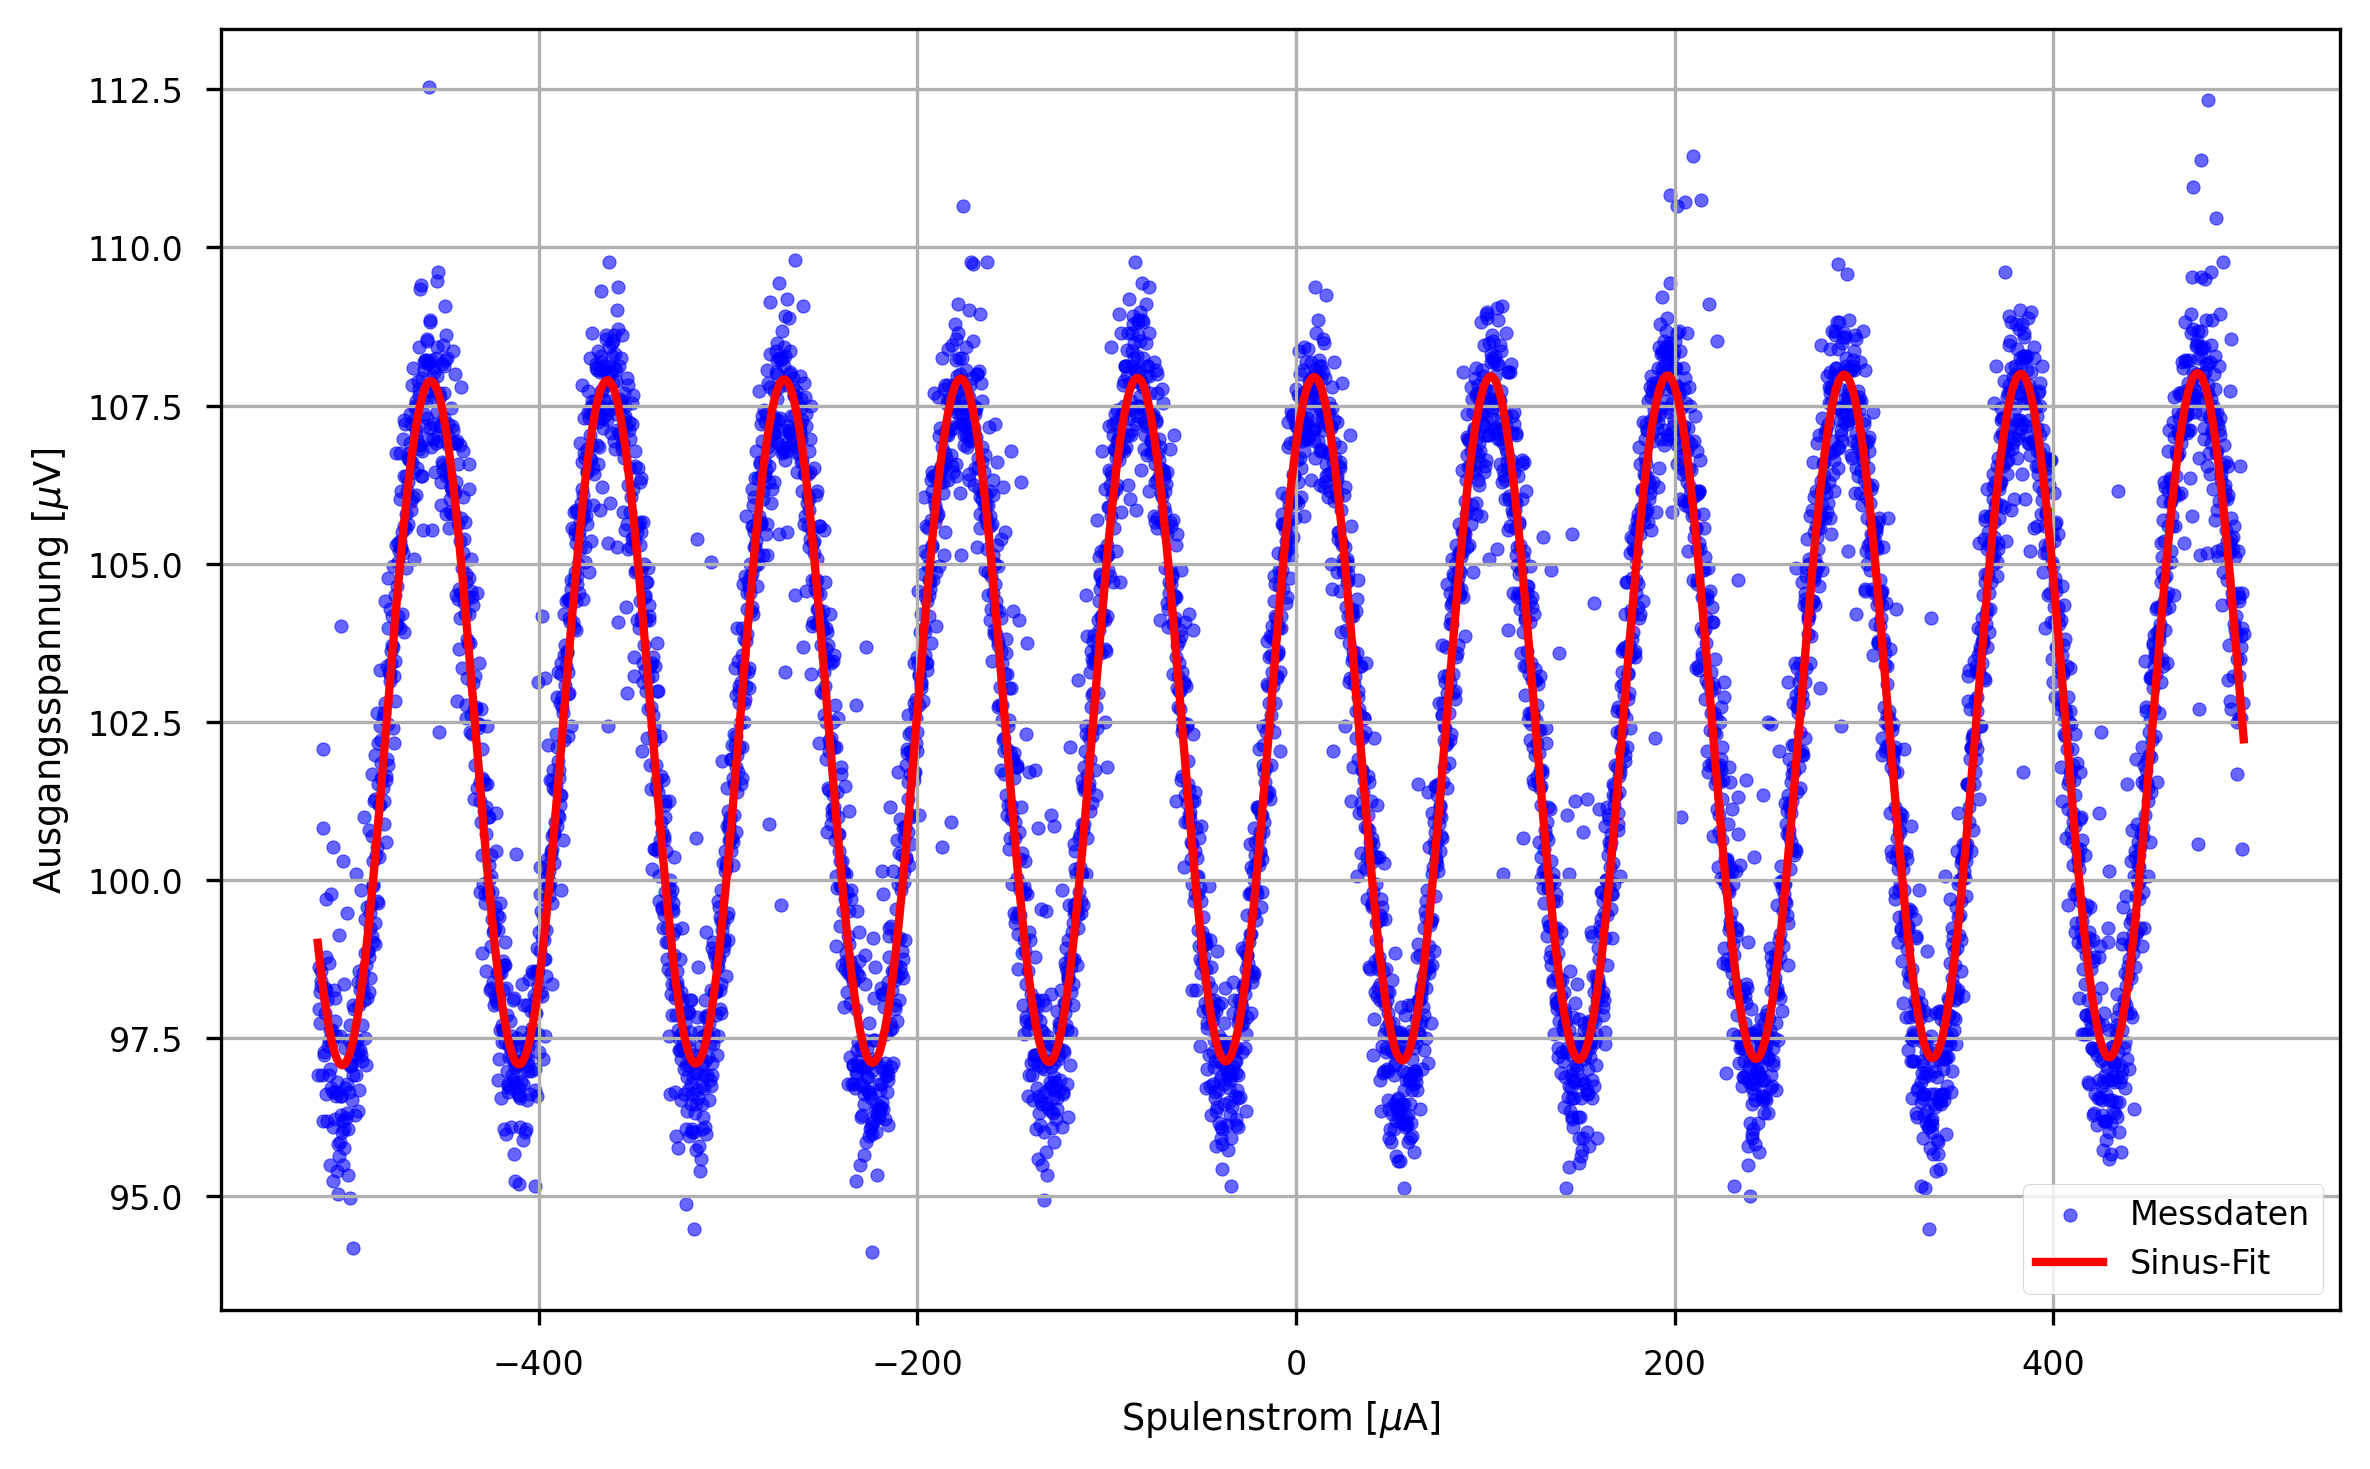
\includegraphics[width=0.75\linewidth]{figures/Aufgabe_D.png}
    \caption{$U_{OUT}$-$I$-Kennlinie des DC-SQUIDs zur $V$-$\Phi$-Charakterisierung. Aufgetragen ist die Ausgangsspannung $U_{OUT}$ gegen den Spulenstrom $I$, der proportional zum magnetischen Fluss $\Phi$ durch den SQUID-Ring ist.}
    \label{fig:aufgabe_d}
\end{figure}

Aus dem Fit ergibt sich für die Periode $\Delta I = 93.3 \pm 0.4 \mathrm{\mu A}$. Als Spannungsmodulation ergab sich $\Delta U = 10.8 \pm 0.2 \mathrm{\mu V}$. Da eine Periode der Änderung des magnetischen Flusses um ein Flussquant entspricht, folgt für die Kopplungsinduktivität

\begin{equation}
    M = \frac{\Phi_0}{\Delta I} = \frac{2.07 \times 10^{-15} \mathrm{Vs}}{93.3 \times 10^{-6} \mathrm{A}} = 2.22 \cdot 10^{-11} \mathrm{H}
\end{equation}

Die Messung zeigt damit die erwartete periodische Abhängigkeit der SQUID-Ausgangsspannung vom magnetischen Fluss. Abweichungen vom ideal sinusförmigen Verlauf lassen sich durch Rauschen, Offsetdrift, eine nicht ideale Einstellung des Arbeitspunktes sowie durch Störungen bei der Flusseinkopplung erklären.

\subsection{Bestimmung von $T_c$ des SQUID Sensors}

\begin{figure}[h]
    \centering
    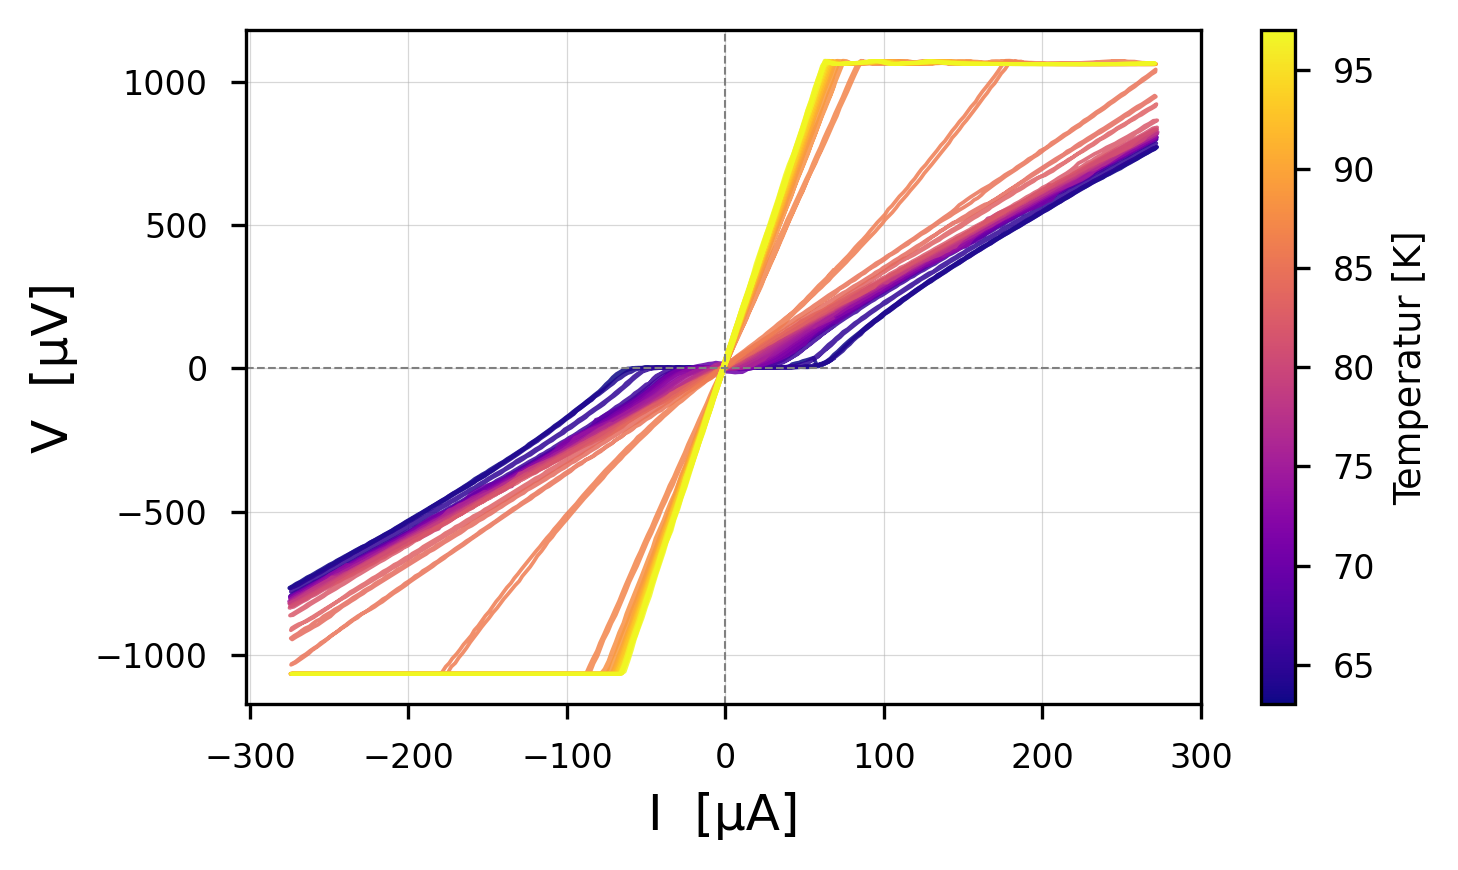
\includegraphics[width=0.75\linewidth]{figures/krit_temp_alle.png}
    \caption{U-I-Kennlinie in Abhängigkeit der Temperatur $T \in [63K, 97K]$ in $1K$ Schritten }
    \label{fig:krit_temp_alle}
\end{figure}

\begin{figure}
    \centering
    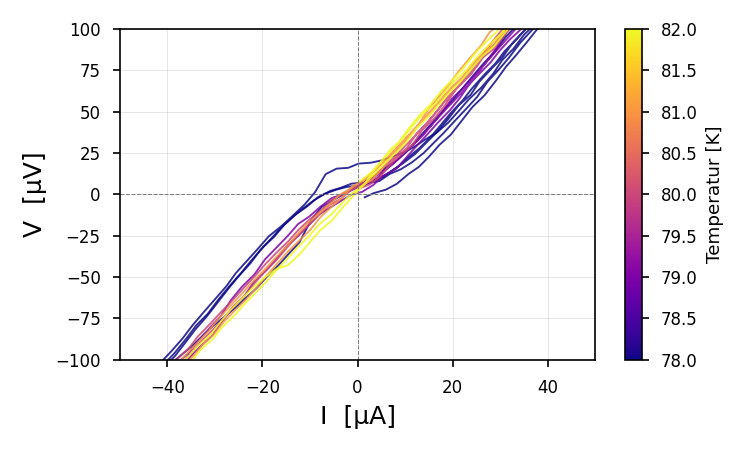
\includegraphics[width=0.75\linewidth]{figures/krit_temp_klein.png}
    \caption{U-I-Kennlinie in Abhängigkeit der Temperatur $T \in [77K, 82K]$ in $1K$ Schritten. Wobei der grobe Schritt von Supraleitender Phase in Normalleitende Phase zu erkenne ist}
    \label{fig:krit_temp_klein}
\end{figure}




\newpage
\listoffigures
\listoftables

%\nocite{*}
\printbibliography

\end{document}
